\section{Problem 2: Simple PRF from DDH}\label{sec:problem2}

Let $\mathbb{G}$ be a cyclic group of prime order $q$ generated by $g \in \mathbb{G}$.
Let $H : \mathcal{M} \rightarrow \mathbb{G}$ be a hash function, which we shall model as a random oracle.
Let $F$ be the PRF defined over $(\mathbb{Z}_{q},\mathcal{M},\mathbb{G})$ as follows:
\begin{equation*}
    F(k,m) \coloneqq H(m)^{k} \hspace{8pt} \text{for } k \in \mathbb{Z}_{q}, m \in \mathcal{M}.
\end{equation*}
Show that $F$ is a secure PRF in the random oracle model for $H$ under the DDH assumption for $\mathbb{G}$.
In particular, you should show that for every adversary $\mathcal{A}$ attacking $F$ as a PRF, there exists a DDH adversary $\mathcal{B}$, which is an elementary wrapper around $\mathcal{A}$, such that $PRFadv[\mathcal{A}, F] \leq DDHadv[\mathcal{B}, \mathbb{G}] + \frac{1}{q}$.

\begin{center}
    \rule{5cm}{0.4pt}
\end{center}

\textbf{\textit{Proof:}}
To solve this exercise we will see that if we can break the PRF game then two distributions are not computationally indistinguishable, and following the result from Exercise 10.10, the DDH assumption does not hold.
In particular, we play the attacker role in the PRF game as defined in \hyperref[ag:4-2]{Attack Game 4.2} and will leverage an adversary for the distinguishing game as defined in \hyperref[ag:3-3]{Attack Game 3.3}.

Let us define define, using the notation from Exercise 10.10, the following variables for the random distributions:
\begin{equation*}
    \begin{split}
        g^{a_i} = H(m) = g^x \text{ for some $x$, } \hspace{3pt} \beta_i = k \in \mathbb{Z}_q, \text{ and } \hspace{3pt} \gamma_i \text{ random}.
    \end{split}
\end{equation*}
The complete scheme is depicted in Figure~\ref{p2:ag}.

\begin{figure}[h!]
    \centering
    \begin{tikzpicture}
        % Define Variables
        \def\lR{0.75}
        \def\rR{5.35}
        \def\lDR{10.75}
        \def\rDR{15.35}
        \def\bottom{-6}

        % Overall Scheme
        \draw[thick] (0,0) -- (6,0) node[midway, anchor=south] {PRF Game $4.2$};
        \node[anchor = north west] at (0,0) (c-r) {\scriptsize Challenger};
        \draw[dotted] (\lR, -0.5) -- (\lR,\bottom);
        \node[anchor = north east, text=red] at (6,0) {\scriptsize Attacker};
        \draw[dotted] (\rR, -0.5) -- (\rR, \bottom);
        \draw[thick, dashed] (6,0) -- (6, \bottom);
        \draw[thick] (10,0) -- (16,0) node[midway, anchor=south] {Distinguishing Game $3.3$};
        \node[anchor = north west, text=red] at (10,0) {\scriptsize Challenger};
        \node[anchor = north east, text=blue] at (16,0) {\scriptsize Attacker};
        \draw[thick, dashed] (10,0) -- (10, \bottom);
        \draw[dotted] (\lDR, -0.5) -- (\lDR, \bottom);
        \draw[dotted] (\rDR, -0.5) -- (\rDR, \bottom);

        % Start Games
        \draw[->] (\rR, -1) -- (\lR, -1) node[midway, anchor=south] {\scriptsize Start Game};
        \node[anchor=west] at (\lR, -1.5) {$b \overset{\mathcal{R}}{\longleftarrow} \{0,1\}$};
        \node[anchor=north west, align=left] at (\lR, -1.75) {\tiny $f \overset{b=0}{\longleftarrow} F(k, \cdot) = H(\cdot)^k = g^{\alpha_i \beta_i}$ \\ \tiny $f \overset{b=1}{\longleftarrow} Funs(\mathcal{X}, \mathcal{Y}) = g^{\gamma_i}$};

        % First Signing Query
        \draw[->] (\rR, -3.25) -- (\lR, -3.25) node[midway, anchor=south] {\scriptsize $Image(m_1)$};
        \node[anchor=south west] at (\lR, -4.25) {$y_1 \leftarrow f(m_1)$};
        \draw[->] (\lR, -4.25) -- (\rR, -4.25) node[anchor=south east] {$y_1$};
        \draw[->,color=red] (\rR, -4.5) -- (\lDR, -4.5) node[midway, anchor=south] {$y_1$};
        \draw[->] (\lDR, -4.75) -- (\rDR, -4.75) node[anchor=south east, text=blue] {$y_1$};

        % Forgery
        \draw[->, thick, color=blue] (\rDR, -5.35) -- (\lDR, -5.35) node[midway, anchor=south] {$\hat{b}$};
        \draw[->, thick, color=red] (\rR, -5.75) -- (\lR, -5.75) node[midway, anchor=south] {$\hat{b} \in \{0,1\}$};
        \draw[->, color=red] (\lDR, -5.5) -- (\rR, -5.5) node[midway, anchor=south, text=red, align=left] {$\hat{b}$};
    \end{tikzpicture}
    \caption{Attack to the $PRF$ game triggering an attacker for the Distinguishing one. In red are the two roles that we actively play, and in black and blue two different entities respectively.\label{p2:ag}}
\end{figure}

Let us consider the following triplet $(g^{x},g^{k}, f(m))$.
Where $g^{x}=H(m)$ for some message, $g^{k}$ is an element of the group $g\in\mathbb{G}$, $k$ the random seed for the PRF game, and $f(m)$ the output of the image query.
\begin{itemize}
    \item If $b = 0$: then $f(m) = g^{xk} = H(m)^k$. 
    \item If $b = 1$: then $f(m)$ is a random element of $\mathbb{G}$.
\end{itemize}
Then the following holds:
\begin{equation*}
    \begin{split}
        \text{PRFadv} & = \left\vert \text{Pr}[W_0] - \text{Pr}[W_1] \right\vert \\
            & = \left\vert Pr(\hat{b}_{PRF} = 1 | b = 0) - Pr(\hat{b}_{PRF} = 1 | b = 1)\right\vert \\
            & = \left\vert Pr(\hat{b}_{PRF} = 1 | b = 0) - Pr(\hat{b}_{PRF} = 1 | b = 1)\right\vert \\
            & = \text{Distadv} \leq \frac{1}{q} + \text{DDHadv}
    \end{split}
\end{equation*}
from where, if the DDH assumption holds and DDHadv is negligible, then so is PRFadv and $F$ is indeed PRF secure. \hfill \qed

